\subsection{Linear Search}

\subsubsection{Code}
\inputminted[]{python}{../Code/linear_search.py}

\subsubsection{Output}
\begin{figure}[!htb]
  \centering
  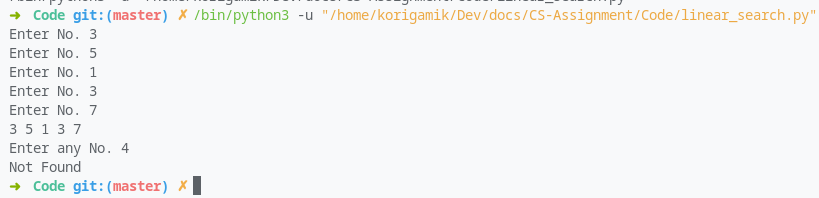
\includegraphics[width=5in]{Images/linear_search.png}
  \label{output:py-1}
  \caption{Output - py - 1}
\end{figure}

\pagebreak

\subsection{Binary Search}

\subsubsection{Code}

\inputminted[]{python}{../Code/binary_search.py}

\subsubsection{Output}
\begin{figure}[!htb]
  \centering
  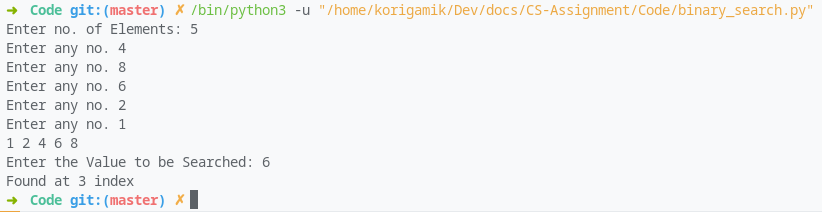
\includegraphics[width=5in]{Images/binary.png}
  \label{output:py-2}
  \caption{Output - py - 2}
\end{figure}
\pagebreak

\subsection{Bubble Sort}

\subsubsection{Code}

\inputminted[]{python}{../Code/bubble_sort.py}

\subsubsection{Output}
\begin{figure}[!htb]
  \centering
  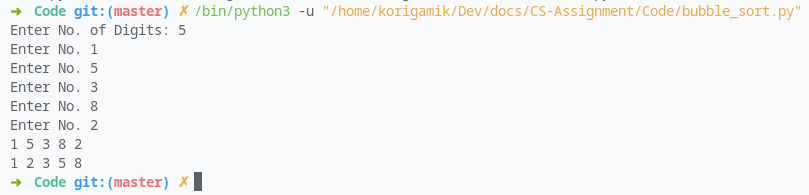
\includegraphics[width=5in]{Images/bubble.png}
  \label{output:py-3}
  \caption{Output - py - 3}
\end{figure}
\pagebreak

\subsection{Selection Sort}

\subsubsection{Code}

\inputminted[]{python}{../Code/selection_sort.py}

\subsubsection{Output}
\begin{figure}[!htb]
  \centering
  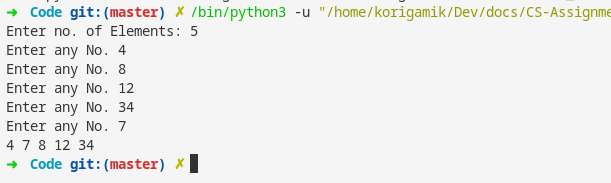
\includegraphics[width=5in]{Images/selection.png}
  \label{output:py-4}
  \caption{Output - py - 4}
\end{figure}
\pagebreak

\subsection{Insertion Sort}

\subsubsection{Code}

\inputminted[]{python}{../Code/insertion_sort.py}

\subsubsection{Output}
\begin{figure}[!htb]
  \centering
  
\includegraphics[width=4in]{Images/insertion.png}
  \label{output:py-5}
  \caption{Output - py - 5}
\end{figure}
\pagebreak

\subsection{Copy File}

\subsubsection{Statement}
Write a Python program to copy from an existing file named “text.txt” to another file “text\_copy.txt”.

\subsubsection{Code}

\inputminted[]{python}{../Code/file_copy.py}

\subsubsection{Output}
\begin{figure}[!htb]
  \centering
  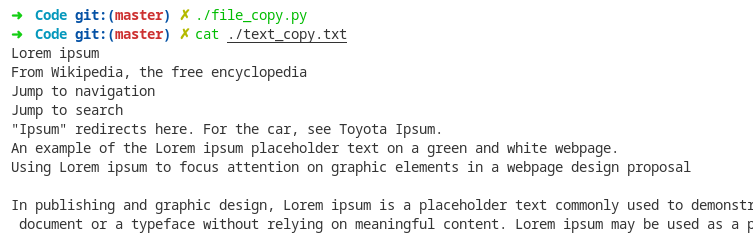
\includegraphics[width=5in]{Images/file_copy.png}
  \label{output:py-6}
  \caption{Output - py - 6}
\end{figure}
\pagebreak

\subsection{Maths}

\newcommand{\oneandcos}{\ensuremath{\sqrt{1+\cos^2\theta}}}

\newcommand{\thetaexpr}{\ensuremath{\sqrt{1+\cos^2\theta}-1}}

\begin{equation} \label{eqn}
  \hspace*{-3.5cm}
  Y_{cm} = \frac{r \tan\theta}{96\pi\cos\theta}
  \bigg(
  \sqrt{2(\thetaexpr)} \bigg(56-5\cos^2\theta+\oneandcos \bigg(1-15\cos^2\theta\Big)\bigg) -
  15\cos^4\theta\bigg(\tan^{-1}\sqrt{\frac{\thetaexpr}{2} + \frac{\pi}{2}}\bigg)
  \bigg)
\end{equation}